\subsection{51 cards}

\renewcommand{\CURPATH}{examples/solitaire/51}

This is a joke I did once for my coworkers who played a Solitaire game too much.
I was wondering, if it's possible to remove some cards, or maybe add (duplicates).

I opened Solitaire.exe in IDA disassembler, which asked if to download PDB file for it from Microsoft servers.
This is usually a rule for many Windows executables and DLLs.
At least, PDB has all function names.

Then I tried to find a 52 number in all functions (because this card game uses 52 cards).
As it turned out, only 2 functions has it.

The first is:

\begin{lstlisting}
.text:00000001000393B4 ; __int64 __fastcall SolitaireGame::OnMoveComplete(SolitaireGame *this)
.text:00000001000393B4 ?OnMoveComplete@SolitaireGame@@QEAAHXZ proc near

...
\end{lstlisting}

The second is the function with self-describing name (name pulled from PDB by IDA): \verb|InitialDeal()|:

\begin{lstlisting}
.text:00000001000365F8 ; void __fastcall SolitaireGame::InitialDeal(SolitaireGame *__hidden this)
.text:00000001000365F8 ?InitialDeal@SolitaireGame@@QEAAXXZ proc near
.text:00000001000365F8
.text:00000001000365F8 var_58          = byte ptr -58h
.text:00000001000365F8 var_48          = qword ptr -48h
.text:00000001000365F8 var_40          = dword ptr -40h
.text:00000001000365F8 var_3C          = dword ptr -3Ch
.text:00000001000365F8 var_38          = dword ptr -38h
.text:00000001000365F8 var_30          = qword ptr -30h
.text:00000001000365F8 var_28          = xmmword ptr -28h
.text:00000001000365F8 var_18          = byte ptr -18h
.text:00000001000365F8
.text:00000001000365F8 ; FUNCTION CHUNK AT .text:00000001000A55C2 SIZE 00000018 BYTES
.text:00000001000365F8
.text:00000001000365F8 ; __unwind { // __CxxFrameHandler3
.text:00000001000365F8                 mov     rax, rsp
.text:00000001000365FB                 push    rdi
.text:00000001000365FC                 push    r12
.text:00000001000365FE                 push    r13
.text:0000000100036600                 sub     rsp, 60h
.text:0000000100036604                 mov     [rsp+78h+var_48], 0FFFFFFFFFFFFFFFEh
.text:000000010003660D                 mov     [rax+8], rbx
.text:0000000100036611                 mov     [rax+10h], rbp
.text:0000000100036615                 mov     [rax+18h], rsi
.text:0000000100036619                 movaps  xmmword ptr [rax-28h], xmm6
.text:000000010003661D                 mov     rsi, rcx
.text:0000000100036620                 xor     edx, edx        ; struct Card *
.text:0000000100036622                 call    ?SetSelectedCard@SolitaireGame@@QEAAXPEAVCard@@@Z ; SolitaireGame::SetSelectedCard(Card *)
.text:0000000100036627                 and     qword ptr [rsi+0F0h], 0
.text:000000010003662F                 mov     rax, cs:?g_pSolitaireGame@@3PEAVSolitaireGame@@EA ; SolitaireGame * g_pSolitaireGame
.text:0000000100036636                 mov     rdx, [rax+48h]
.text:000000010003663A                 cmp     byte ptr [rdx+51h], 0
.text:000000010003663E                 jz      short loc_10003664E
.text:0000000100036640                 xor     r8d, r8d        ; bool
.text:0000000100036643                 mov     dl, 1           ; int
.text:0000000100036645                 lea     ecx, [r8+3]     ; this
.text:0000000100036649                 call    ?PlaySoundProto@GameAudio@@YA_NH_NPEAI@Z ; GameAudio::PlaySoundProto(int,bool,uint *)
.text:000000010003664E
.text:000000010003664E loc_10003664E:                          ; CODE XREF: SolitaireGame::InitialDeal(void)+46
.text:000000010003664E                 mov     rbx, [rsi+88h]
.text:0000000100036655                 mov     r8d, 4
.text:000000010003665B                 lea     rdx, aCardstackCreat ; "CardStack::CreateDeck()::uiNumSuits == "...
.text:0000000100036662                 mov     ebp, 10000h
.text:0000000100036667                 mov     ecx, ebp        ; unsigned int
.text:0000000100036669                 call    ?Log@@YAXIPEBGZZ ; Log(uint,ushort const *,...)
.text:000000010003666E                 mov     r8d, 52         ; ---
.text:0000000100036674                 lea     rdx, aCardstackCreat_0 ; "CardStack::CreateDeck()::uiNumCards == "...
.text:000000010003667B                 mov     ecx, ebp        ; unsigned int
.text:000000010003667D                 call    ?Log@@YAXIPEBGZZ ; Log(uint,ushort const *,...)
.text:0000000100036682                 xor     edi, edi

.text:0000000100036684 loc_100036684:                          ; CODE XREF: SolitaireGame::InitialDeal(void)+C0
.text:0000000100036684                 mov     eax, 4EC4EC4Fh
.text:0000000100036689                 mul     edi
.text:000000010003668B                 mov     r8d, edx
.text:000000010003668E                 shr     r8d, 4          ; unsigned int
.text:0000000100036692                 mov     eax, r8d
.text:0000000100036695                 imul    eax, 52         ; ---
.text:0000000100036698                 mov     edx, edi
.text:000000010003669A                 sub     edx, eax        ; unsigned int
.text:000000010003669C                 mov     rcx, [rbx+128h] ; this
.text:00000001000366A3                 call    ?CreateCard@CardTable@@IEAAPEAVCard@@II@Z ; CardTable::CreateCard(uint,uint)
.text:00000001000366A8                 mov     rdx, rax        ; struct Card *
.text:00000001000366AB                 mov     rcx, rbx        ; this
.text:00000001000366AE                 call    ?Push@CardStack@@QEAAXPEAVCard@@@Z ; CardStack::Push(Card *)
.text:00000001000366B3                 inc     edi
.text:00000001000366B5                 cmp     edi, 52         ; ---
.text:00000001000366B8                 jb      short loc_100036684

.text:00000001000366BA                 xor     r8d, r8d        ; bool
.text:00000001000366BD                 xor     edx, edx        ; bool
.text:00000001000366BF                 mov     rcx, rbx        ; this
.text:00000001000366C2                 call    ?Arrange@CardStack@@QEAAX_N0@Z ; CardStack::Arrange(bool,bool)
.text:00000001000366C7                 mov     r13, [rsi+88h]
.text:00000001000366CE                 lea     rdx, aCardstackShuff ; "CardStack::Shuffle()"
.text:00000001000366D5                 mov     ecx, ebp        ; unsigned int
.text:00000001000366D7                 call    ?Log@@YAXIPEBGZZ ; Log(uint,ushort const *,...)
.text:00000001000366DC                 and     [rsp+78h+var_40], 0
.text:00000001000366E1                 and     [rsp+78h+var_3C], 0
.text:00000001000366E6                 mov     [rsp+78h+var_38], 10h
.text:00000001000366EE                 xor     ebx, ebx
.text:00000001000366F0                 mov     [rsp+78h+var_30], rbx

...
\end{lstlisting}

Anyway, we clearly see a loop of 52 iterations.
A loop body has calls to \verb|CardTable()::CreateCard()| and \verb|CardStack::Push()|.

The \verb|CardTable::CreateCard()| eventually calls \verb|Card::Init()| with values in 0..51 range, as one of its arguments.
This can be easily checked using debugger.

So I tried just to change the 52 (0x34) number to 51 (0x33) in the \TT{cmp edi, 52} instruction at \TT{0x1000366B5} and run it.
At first glance, nothing happened, but I noticed that now it's hard to solve the game.
I spent almost an hour to reach this \textit{position}:

\begin{figure}[H]
\centering
\frame{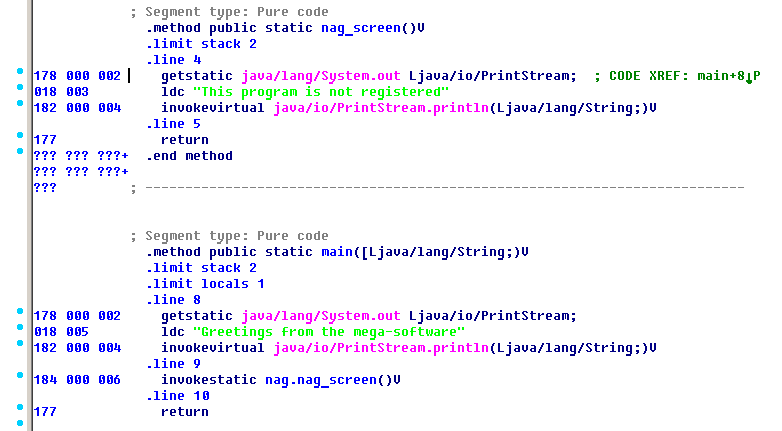
\includegraphics[width=\textwidth]{\CURPATH/1.png}}
\end{figure}

Ace of hearts is missing. Perhaps, internally, this card is numbered as 51th (if to number them from zero).

In the other place I found all card names. Maybe names to be used to fetch card graphics from resources?

\begin{lstlisting}
.data:00000001000B6970 ?CARD_NAME@Card@@2PAPEBGA dq offset aTwoofclubs
.data:00000001000B6970                                         ; "TwoOfClubs"
.data:00000001000B6978                 dq offset aThreeofclubs ; "ThreeOfClubs"
.data:00000001000B6980                 dq offset aFourofclubs  ; "FourOfClubs"
.data:00000001000B6988                 dq offset aFiveofclubs  ; "FiveOfClubs"
.data:00000001000B6990                 dq offset aSixofclubs   ; "SixOfClubs"
.data:00000001000B6998                 dq offset aSevenofclubs ; "SevenOfClubs"
.data:00000001000B69A0                 dq offset aEightofclubs ; "EightOfClubs"
.data:00000001000B69A8                 dq offset aNineofclubs  ; "NineOfClubs"
.data:00000001000B69B0                 dq offset aTenofclubs   ; "TenOfClubs"
.data:00000001000B69B8                 dq offset aJackofclubs  ; "JackOfClubs"
.data:00000001000B69C0                 dq offset aQueenofclubs ; "QueenOfClubs"
.data:00000001000B69C8                 dq offset aKingofclubs  ; "KingOfClubs"
.data:00000001000B69D0                 dq offset aAceofclubs   ; "AceOfClubs"
.data:00000001000B69D8                 dq offset aTwoofdiamonds ; "TwoOfDiamonds"
.data:00000001000B69E0                 dq offset aThreeofdiamond ; "ThreeOfDiamonds"
.data:00000001000B69E8                 dq offset aFourofdiamonds ; "FourOfDiamonds"
.data:00000001000B69F0                 dq offset aFiveofdiamonds ; "FiveOfDiamonds"
.data:00000001000B69F8                 dq offset aSixofdiamonds ; "SixOfDiamonds"
.data:00000001000B6A00                 dq offset aSevenofdiamond ; "SevenOfDiamonds"
.data:00000001000B6A08                 dq offset aEightofdiamond ; "EightOfDiamonds"
.data:00000001000B6A10                 dq offset aNineofdiamonds ; "NineOfDiamonds"
.data:00000001000B6A18                 dq offset aTenofdiamonds ; "TenOfDiamonds"
.data:00000001000B6A20                 dq offset aJackofdiamonds ; "JackOfDiamonds"
.data:00000001000B6A28                 dq offset aQueenofdiamond ; "QueenOfDiamonds"
.data:00000001000B6A30                 dq offset aKingofdiamonds ; "KingOfDiamonds"
.data:00000001000B6A38                 dq offset aAceofdiamonds ; "AceOfDiamonds"
.data:00000001000B6A40                 dq offset aTwoofspades  ; "TwoOfSpades"
.data:00000001000B6A48                 dq offset aThreeofspades ; "ThreeOfSpades"
.data:00000001000B6A50                 dq offset aFourofspades ; "FourOfSpades"
.data:00000001000B6A58                 dq offset aFiveofspades ; "FiveOfSpades"
.data:00000001000B6A60                 dq offset aSixofspades  ; "SixOfSpades"
.data:00000001000B6A68                 dq offset aSevenofspades ; "SevenOfSpades"
.data:00000001000B6A70                 dq offset aEightofspades ; "EightOfSpades"
.data:00000001000B6A78                 dq offset aNineofspades ; "NineOfSpades"
.data:00000001000B6A80                 dq offset aTenofspades  ; "TenOfSpades"
.data:00000001000B6A88                 dq offset aJackofspades ; "JackOfSpades"
.data:00000001000B6A90                 dq offset aQueenofspades ; "QueenOfSpades"
.data:00000001000B6A98                 dq offset aKingofspades ; "KingOfSpades"
.data:00000001000B6AA0                 dq offset aAceofspades  ; "AceOfSpades"
.data:00000001000B6AA8                 dq offset aTwoofhearts  ; "TwoOfHearts"
.data:00000001000B6AB0                 dq offset aThreeofhearts ; "ThreeOfHearts"
.data:00000001000B6AB8                 dq offset aFourofhearts ; "FourOfHearts"
.data:00000001000B6AC0                 dq offset aFiveofhearts ; "FiveOfHearts"
.data:00000001000B6AC8                 dq offset aSixofhearts  ; "SixOfHearts"
.data:00000001000B6AD0                 dq offset aSevenofhearts ; "SevenOfHearts"
.data:00000001000B6AD8                 dq offset aEightofhearts ; "EightOfHearts"
.data:00000001000B6AE0                 dq offset aNineofhearts ; "NineOfHearts"
.data:00000001000B6AE8                 dq offset aTenofhearts  ; "TenOfHearts"
.data:00000001000B6AF0                 dq offset aJackofhearts ; "JackOfHearts"
.data:00000001000B6AF8                 dq offset aQueenofhearts ; "QueenOfHearts"
.data:00000001000B6B00                 dq offset aKingofhearts ; "KingOfHearts"
.data:00000001000B6B08                 dq offset aAceofhearts  ; "AceOfHearts"

.data:00000001000B6B10 ; public: static unsigned short const * near * Card::CARD_HUMAN_NAME
.data:00000001000B6B10 ?CARD_HUMAN_NAME@Card@@2PAPEBGA dq offset a54639Cardnames
.data:00000001000B6B10                                         ; "|54639|CardNames|Two Of Clubs"
.data:00000001000B6B18                 dq offset a64833Cardnames ; "|64833|CardNames|Three Of Clubs"
.data:00000001000B6B20                 dq offset a62984Cardnames ; "|62984|CardNames|Four Of Clubs"
.data:00000001000B6B28                 dq offset a65200Cardnames ; "|65200|CardNames|Five Of Clubs"
.data:00000001000B6B30                 dq offset a52967Cardnames ; "|52967|CardNames|Six Of Clubs"
.data:00000001000B6B38                 dq offset a42781Cardnames ; "|42781|CardNames|Seven Of Clubs"
.data:00000001000B6B40                 dq offset a49217Cardnames ; "|49217|CardNames|Eight Of Clubs"
.data:00000001000B6B48                 dq offset a44682Cardnames ; "|44682|CardNames|Nine Of Clubs"
.data:00000001000B6B50                 dq offset a51853Cardnames ; "|51853|CardNames|Ten Of Clubs"
.data:00000001000B6B58                 dq offset a46368Cardnames ; "|46368|CardNames|Jack Of Clubs"
.data:00000001000B6B60                 dq offset a61344Cardnames ; "|61344|CardNames|Queen Of Clubs"
.data:00000001000B6B68                 dq offset a65017Cardnames ; "|65017|CardNames|King Of Clubs"
.data:00000001000B6B70                 dq offset a57807Cardnames ; "|57807|CardNames|Ace Of Clubs"
.data:00000001000B6B78                 dq offset a48455Cardnames ; "|48455|CardNames|Two Of Diamonds"
.data:00000001000B6B80                 dq offset a44156Cardnames ; "|44156|CardNames|Three Of Diamonds"
.data:00000001000B6B88                 dq offset a51672Cardnames ; "|51672|CardNames|Four Of Diamonds"
.data:00000001000B6B90                 dq offset a45972Cardnames ; "|45972|CardNames|Five Of Diamonds"
.data:00000001000B6B98                 dq offset a47206Cardnames ; "|47206|CardNames|Six Of Diamonds"
.data:00000001000B6BA0                 dq offset a48399Cardnames ; "|48399|CardNames|Seven Of Diamonds"
.data:00000001000B6BA8                 dq offset a47847Cardnames ; "|47847|CardNames|Eight Of Diamonds"
.data:00000001000B6BB0                 dq offset a48606Cardnames ; "|48606|CardNames|Nine Of Diamonds"
.data:00000001000B6BB8                 dq offset a61278Cardnames ; "|61278|CardNames|Ten Of Diamonds"
.data:00000001000B6BC0                 dq offset a52038Cardnames ; "|52038|CardNames|Jack Of Diamonds"
.data:00000001000B6BC8                 dq offset a54643Cardnames ; "|54643|CardNames|Queen Of Diamonds"
.data:00000001000B6BD0                 dq offset a48902Cardnames ; "|48902|CardNames|King Of Diamonds"
.data:00000001000B6BD8                 dq offset a46672Cardnames ; "|46672|CardNames|Ace Of Diamonds"
.data:00000001000B6BE0                 dq offset a41049Cardnames ; "|41049|CardNames|Two Of Spades"
.data:00000001000B6BE8                 dq offset a49327Cardnames ; "|49327|CardNames|Three Of Spades"
.data:00000001000B6BF0                 dq offset a51933Cardnames ; "|51933|CardNames|Four Of Spades"
.data:00000001000B6BF8                 dq offset a42651Cardnames ; "|42651|CardNames|Five Of Spades"
.data:00000001000B6C00                 dq offset a65342Cardnames ; "|65342|CardNames|Six Of Spades"
.data:00000001000B6C08                 dq offset a53644Cardnames ; "|53644|CardNames|Seven Of Spades"
.data:00000001000B6C10                 dq offset a54466Cardnames ; "|54466|CardNames|Eight Of Spades"
.data:00000001000B6C18                 dq offset a56874Cardnames ; "|56874|CardNames|Nine Of Spades"
.data:00000001000B6C20                 dq offset a46756Cardnames ; "|46756|CardNames|Ten Of Spades"
.data:00000001000B6C28                 dq offset a62876Cardnames ; "|62876|CardNames|Jack Of Spades"
.data:00000001000B6C30                 dq offset a64633Cardnames ; "|64633|CardNames|Queen Of Spades"
.data:00000001000B6C38                 dq offset a46215Cardnames ; "|46215|CardNames|King Of Spades"
.data:00000001000B6C40                 dq offset a60450Cardnames ; "|60450|CardNames|Ace Of Spades"
.data:00000001000B6C48                 dq offset a51010Cardnames ; "|51010|CardNames|Two Of Hearts"
.data:00000001000B6C50                 dq offset a64948Cardnames ; "|64948|CardNames|Three Of Hearts"
.data:00000001000B6C58                 dq offset a43079Cardnames ; "|43079|CardNames|Four Of Hearts"
.data:00000001000B6C60                 dq offset a57131Cardnames ; "|57131|CardNames|Five Of Hearts"
.data:00000001000B6C68                 dq offset a58953Cardnames ; "|58953|CardNames|Six Of Hearts"
.data:00000001000B6C70                 dq offset a45105Cardnames ; "|45105|CardNames|Seven Of Hearts"
.data:00000001000B6C78                 dq offset a47775Cardnames ; "|47775|CardNames|Eight Of Hearts"
.data:00000001000B6C80                 dq offset a41825Cardnames ; "|41825|CardNames|Nine Of Hearts"
.data:00000001000B6C88                 dq offset a41501Cardnames ; "|41501|CardNames|Ten Of Hearts"
.data:00000001000B6C90                 dq offset a47108Cardnames ; "|47108|CardNames|Jack Of Hearts"
.data:00000001000B6C98                 dq offset a55659Cardnames ; "|55659|CardNames|Queen Of Hearts"
.data:00000001000B6CA0                 dq offset a44572Cardnames ; "|44572|CardNames|King Of Hearts"
.data:00000001000B6CA8                 dq offset a44183Cardnames ; "|44183|CardNames|Ace Of Hearts"
\end{lstlisting}

If you want to do this to someone, be sure his/her mental health is stable.

Aside of function names from PDB file, there are lots of \verb|Log()| function calls that can help significantly,
because the Solitaire game reports about what it's doing right now.

Homework: try to \textit{remove} several cards or two of clubs.
And what if to swap card names in arrays of strings?

I also tried to pass a numbers like 0, 0..50 to \verb|Card:Init()| (so to have 2 zeroes in a list of 52 numbers).
Then I saw two \textit{two of clubs} cards at one moment, but Solitaire behaves erratically.

This is patched Windows 7 Solitare:
\href{\RepoURL/examples/solitaire/51/Solitaire51.exe}{Solitaire51.exe}.

